% Recovery and information chapters. All labels and citation keys are prefixed rec: / Rec.
% This fragment deliberately uses only ordinary theorem environments and amsmath.
\section{What the relationships remember}\label{rec:relationships}

The curve led us to $K(k)$, the limiting probability that $k$ sampled
integers are pairwise coprime. Let us reverse that experiment. Hide the
integers and keep only the coprimality answers. A single answer contains
very little: ``not coprime'' does not say whether the common divisor is
$2$, $7$, or $1009$. A whole collection of answers contains much more.
It can identify the \emph{actual numerical primes} shared by a pair.

Here are the rules of the finite game we shall eventually play.
\begin{enumerate}
 \item Put independent uniform integers from $1$ to $N^2$ in $N$
 numbered boxes. The box numbers remain visible; the contents are hidden.
 \item For each pair, write one bit: $1$ if the contents are coprime,
 and $0$ otherwise. Independently reverse each bit with the same unknown
 probability.
 \item Give the resulting table to a decoder. Its task is to name every
 prime shared by each pair of boxes, with a fraction of mistaken pairs
 tending to zero as the experiment grows.
\end{enumerate}
There is just one observed bit per pair. The decoder cannot ask for a
second, cleaner answer. We will allow the error probability to approach
one half, making individual answers approach fair coin tosses.

Before introducing noise, we can see the arithmetic mechanism in three
ordinary fractions.

\subsection{Three percentages name the shared primes}

Temporarily open two boxes and put $210$ and $462$ inside them. Test each
against a third integer chosen uniformly from $1$ to $M$, and let
$M\to\infty$. The exact limiting frequencies are
\[
\begin{array}{c|c}
 \text{the third integer is coprime to} & \text{frequency}\\ \hline
 210=2\cdot3\cdot5\cdot7 & 8/35\\[2pt]
 462=2\cdot3\cdot7\cdot11 & 20/77\\[2pt]
 \text{both} & 16/77
\end{array}
\]
For the last row it must avoid $2,3,5,7,11$. Multiply the first two
frequencies and divide by the third:
\[
 \frac{(8/35)(20/77)}{16/77}
 =\frac27
 =\left(1-\frac12\right)
  \left(1-\frac13\right)
  \left(1-\frac17\right).
\]
The factors belonging to $5$ and $11$ cancel. Each belongs to one box,
so it occurs once above and once below. A shared prime occurs twice
above and once below, leaving one factor behind. Closing the boxes
again does not change the calculation: the three frequencies alone
identify the common-prime product.

There is a second small surprise. The reduced fraction $2/7$ has hidden
the primes $2$ and $3$ through ordinary cancellation, but has not lost
them. Its denominator gives away $7$; removing the factor $6/7$ exposes
the next prime:
\[
 \frac27\ \xrightarrow{\ \times7/6\ }\ \frac13
 \ \xrightarrow{\ \times3/2\ }\ \frac12
 \ \xrightarrow{\ \times2\ }\ 1.
\]
Thus the three percentages recover the entire set $\{2,3,7\}$.

\begin{lemma}[Reading a finite prime set from a rational number]
\label{rec:totient-decoder}
For a finite set $A$ of primes, the rational number
$q(A)=\prod_{p\in A}(p-1)/p$ determines $A$ uniquely. If $A$ is nonempty,
its largest prime is the largest prime factor of the denominator of
$q(A)$ in lowest terms. Remove this prime $p$ by multiplying the ratio
by $p/(p-1)$, and repeat until the ratio is one.
\end{lemma}
\begin{proof}
Let $p=\max A$. No numerator factor $r-1$, with $r\in A$, is divisible
by $p$, so $p$ remains in the reduced denominator. No larger prime
can occur there. Removing the factor $(p-1)/p$ reduces the question
to a smaller set.
\end{proof}
This is the classical injectivity of the totient ratio on squarefree
integers; Tao~\cite[Lemma~2.1 and Remark~2.3]{RecTaoTotient2024} records
the same descending-prime mechanism. We will use it as a decoder.

\subsection{A rational relation among transcendental frequencies}

To turn the three percentages into observable quantities, give each box
infinitely many independent reference boxes. The natural limiting model
keeps only prime divisibility. At prime $p$, a box contains that feature
with probability $1/p$; all these choices are independent.

For each vertex $i\ge1$ and prime $p$, independently let
$B_{i,p}$ have Bernoulli distribution with parameter $1/p$. Write
$S_i=\{p:B_{i,p}=1\}$ and join $i$ to $j$ when $S_i\cap S_j$ is empty.
We denote this answer by $E_{ij}$, and put $E_{ii}=0$.
These are the prime-divisibility profiles of independent Haar-random
profinite integers. No profinite terminology is needed for the arguments:
the independent bits just specified define the entire model. Each box
carries infinitely many primes almost surely, by independence and the
divergence of $\sum_p1/p$. Two boxes share only finitely many almost
surely, since $\sum_p1/p^2$ converges. That difference between a single
profile and a shared profile is what makes a finite rational answer
possible.

For a fixed number of sampled ordinary integers, their coprimality graph
converges to this model as the sampling range tends to infinity. Indeed,
the Chinese remainder theorem gives convergence of every fixed finite
prime profile. For $k$ vertices, ignoring primes above $R$ changes some
edge with probability at most $\binom{k}{2}\sum_{p>R}p^{-2}$, in either
model. First take the range limit and then $R\to\infty$.
This prime-feature description belongs to the established probabilistic
theory of coprimality; see, for example, Martineau~\cite{RecMartineauVisibility2019}.

The familiar kernel has a direct interpretation here:
\begin{equation}\label{rec:clique-kernel}
 \Prob(E_{ij}=1\text{ for all }1\le i<j\le k)
 =\prod_p(1-1/p)^{k-1}\bigl(1+(k-1)/p\bigr)=K(k).
\end{equation}
At each prime, at most one of the $k$ profiles may contain it. In
particular the edge probability is
\begin{equation}\label{rec:kappa}
 \kappa=K(2)=\prod_p(1-p^{-2})=\frac6{\pi^2}.
\end{equation}
Thus the same $K$ that determined the moments of the prime probability
law now describes a sampling experiment.

For a fixed box, let $d_i$ be the fraction of reference boxes coprime to
it. For two boxes, let $c_{ij}$ be the fraction coprime to both. Formally,
\[
 d_i=\lim_{M\to\infty}\frac1M\sum_{k\le M}E_{ik},\qquad
 c_{ij}=\lim_{M\to\infty}\frac1M\sum_{k\le M}E_{ik}E_{jk}.
\]
The omitted diagonal terms have no effect on these limits. The same
cancellation as in the example survives even though each individual
profile now contains infinitely many primes almost surely.

\begin{theorem}[Frequency reconstruction]\label{rec:frequency}
Almost surely all $d_i,c_{ij}$ exist and are positive, every pair shares
only finitely many primes, and
\begin{equation}\label{rec:ratio}
 \frac{d_i d_j}{c_{ij}}
 =\prod_{p\in S_i\cap S_j}\left(1-\frac1p\right).
\end{equation}
Consequently the ordered infinite graph determines every set $S_i$,
including the numerical labels of its primes. The random variables
$d_1,d_2,\ldots$ are almost surely algebraically independent over
$\mathbb Q$, and each $c_{ij}$ is almost surely transcendental.
\end{theorem}
\begin{proof}
Tonelli's theorem gives
$\E\sum_{p\in S_i}p^{-1}=\sum_p p^{-2}<\infty$. Thus, almost surely,
the following products converge to positive values. Conditional strong
laws, with the displayed profiles held fixed, give
\begin{equation}\label{rec:degree-products}
 d_i=\prod_{p\in S_i}(1-1/p),\qquad
 c_{ij}=\prod_{p\in S_i\cup S_j}(1-1/p).
\end{equation}
Also $\E|S_i\cap S_j|=\sum_p p^{-2}<\infty$, so the intersection is
finite almost surely. Cancelling the convergent logarithms in
\eqref{rec:degree-products} proves \eqref{rec:ratio}, and
Lemma~\ref{rec:totient-decoder} recovers each intersection. Every prime
present in $S_i$ occurs in infinitely many other profiles almost surely,
so their intersections recover all of $S_i$. Countability makes these
assertions simultaneous for all vertices and primes.

For the last assertions consider
$Z=\prod_p(1-1/p)^{C_p}$, where independent $C_p$ have parameters
$q_p=1/p$ or $q_p=2/p-1/p^2$. Both products converge positively by the
same argument. By Lemma~\ref{rec:totient-decoder}, distinct assignments
of the bits through $R$ give distinct prefix products. The largest
prefix atom is therefore
\[
 M_R=\prod_{p\le R}\max(q_p,1-q_p)\longrightarrow0,
\]
since $\sum_p\min(q_p,1-q_p)=\infty$. Conditional on the independent
positive tail, the probability that the whole product equals any
specified real number is at most $M_R$. Hence $Z$ has no atoms. This
applies to $d_i$ and $c_{ij}$, and the countability of algebraic numbers
proves their almost-sure transcendence.

The $d_i$ are independent. A nonzero polynomial in finitely many of
them vanishes with probability zero: induct on the number of variables,
condition on all but the last, and use the finitely many roots of the
remaining nonzero one-variable polynomial. Taking the countable union
over rational polynomials proves algebraic independence.
\end{proof}

The single-box frequencies $d_i$ are almost surely algebraically
independent: no nonzero polynomial with rational coefficients vanishes
at any finite list of them. Each common-neighbor frequency is also
transcendental. Yet multiplying the two individual frequencies and
dividing by the joint frequency gives an exact rational code for the
shared primes. The arithmetic is in the dependence between the
observations. None of the three percentages needs to be rational for
their combination to name $2$, $3$, and $7$.

For a fixed box, every prime it contains eventually appears in another
box. Taking the union of the recovered intersections therefore recovers
its entire prime profile. This is a statement about the random infinite
experiment; it supplies almost-sure transcendence, rather than an
explicit new named transcendental number. The visible box labels keep
the sampling order needed to form the frequencies.

\subsection{Calibrating a corrupted infinite table}

Now corrupt the answers. There is initially an extra unknown: a low
observed coprimality frequency might reflect arithmetic or a tendency
of the channel to reverse answers. The average over the whole table
separates them. Its clean value is already known, $6/\pi^2$, so the
same constant that counted coprime pairs calibrates the noise.

Suppose each unordered answer is independently flipped with a fixed
probability $\varepsilon$, independently of the profiles. Put
$a=1-2\varepsilon$. The corrupted neighbor and common-neighbor
frequencies $u_i,v_{ij}$ satisfy
\begin{equation}\label{rec:infinite-noise}
 u_i=\varepsilon+a d_i,\qquad
 v_{ij}=\varepsilon^2+\varepsilon a(d_i+d_j)+a^2c_{ij}.
\end{equation}
The limiting edge density $q$ is
$q=\varepsilon+a\kappa$, so the unknown error rate is recovered by
\begin{equation}\label{rec:epsilon}
 \varepsilon=\frac{\kappa-q}{2\kappa-1}.
\end{equation}
The denominator is nonzero. The conditional strong law proves
\eqref{rec:infinite-noise}; the edge-density strong law follows from
bounded differences in the independent vertex profiles and then in the
independent edge flips. For example the resulting exponentially small
tail probabilities are summable, so Borel--Cantelli applies.

If $a\ne0$, equations \eqref{rec:infinite-noise} recover $d_i,c_{ij}$,
then all prime profiles by Theorem~\ref{rec:frequency}. An error rate
above one half is still usable: for example, an answer that is always
reversed can simply be reversed again. The calibration discovers which
side of one half we are on. Exactly at one half, every observed answer
is an independent fair coin and all arithmetic information disappears.
An arbitrarily small fixed distance from one half can be overcome by
infinitely many boxes. The finite game asks how small that distance
may become as the number of boxes grows.

\section{The recovery paradox}\label{rec:paradox-section}

Return now to the finite boxes. The exact ratio is no longer available:
we have estimated frequencies, corrupted observations, and only finitely
many reference boxes. We must explain how an approximation to a real
number can still reveal an exact prime set. The proof uses the repeated
patterns across the whole table to strengthen its frequency estimates.

For each $N$, independently sample $X_1,\ldots,X_N$ uniformly from
$\{1,\ldots,N^2\}$. Let $G_N$ be the labelled coprimality graph with
adjacency matrix $E$, and observe
\begin{equation}\label{rec:finite-model}
 Y_{ij}=E_{ij}\mathbin{\oplus}A_{ij},\qquad
 A_{ij}\sim\operatorname{Bernoulli}(\varepsilon_N),\quad i<j.
\end{equation}
All flips are mutually independent and independent of the integers.
The common error probability is unknown to the recovery algorithm and
may vary with $N$; $\oplus$ denotes addition modulo two. Write
\begin{equation}\label{rec:signal}
 \begin{aligned}
 a_N&=1-2\varepsilon_N, & T_N&=Na_N^2,\\
 R_{ij}&=\rad\gcd(X_i,X_j).
 \end{aligned}
\end{equation}
The quantity $a_N$ is the signed strength of one answer; $T_N$ combines
that strength with the number of available boxes. The integer $R_{ij}$
records every shared prime once. For the pair $210,462$, it equals
$42=2\cdot3\cdot7$. Coprimality does not record prime-power exponents.

\begin{figure}[tb]
 \centering
 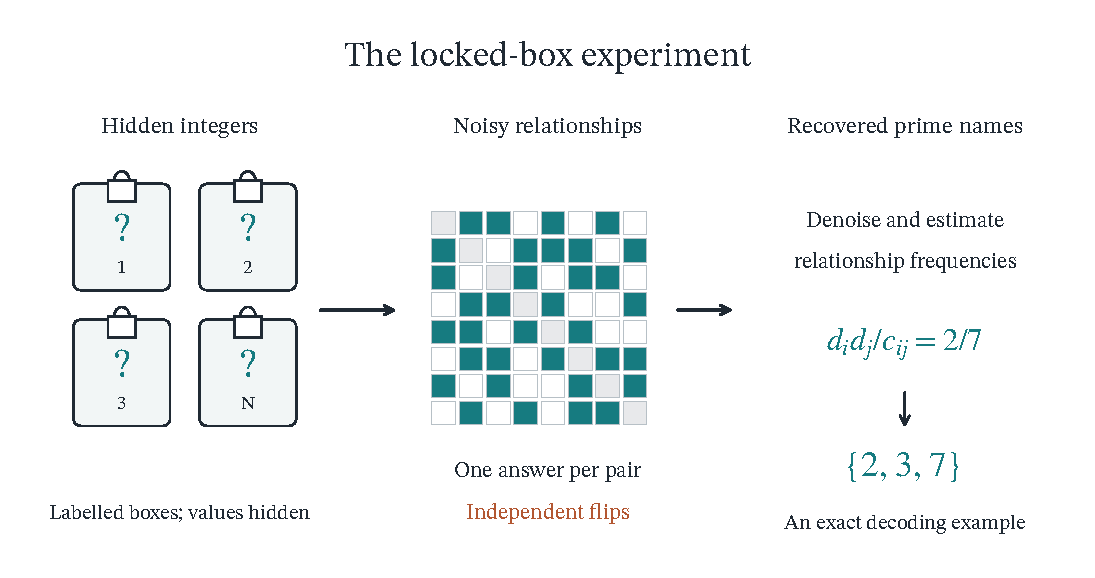
\includegraphics[width=\linewidth]{figures/04_locked_boxes.pdf}
 \caption{A schematic of the recovery experiment. The box identities
 remain aligned while their integer values are hidden. One independently
 corrupted coprimality bit is observed per unordered pair. The theorem
 recovers exact shared-prime sets on a fraction of pairs tending to one;
 this diagram makes no finite-sample accuracy claim. The exact ratio
 $2/7$ illustrates the decoder for the prime set $\{2,3,7\}$.}
 \label{rec:locked-boxes-figure}
\end{figure}

\begin{theorem}[The threshold for recovery on almost every pair]\label{rec:threshold}
There is a single procedure using $Y$ alone such that, whenever
$T_N\to\infty$, for every fixed pair $i\ne j$,
\[
 \Prob(\widehat R_{ij}=R_{ij})\longrightarrow1,
 \qquad
 \frac1{\binom N2}\sum_{i<j}\mathbf1_{\{\widehat R_{ij}\ne R_{ij}\}}
 \longrightarrow0\quad\hbox{in probability}.
\]
If $T_N$ does not tend to infinity, neither a vanishing error probability
for a fixed pair nor a vanishing fraction of pair errors is possible,
even if $\varepsilon_N$ is supplied. The same criterion holds in the
independent-prime model.
\end{theorem}

This is a sharp distinction. If the distance of the error rate from one
half is a constant times $N^{-1/2}$, some uncertainty about a fixed
pair persists. Multiply that distance by \emph{any} factor tending to
infinity, however slowly, and consistency becomes possible. The theorem
names the primes correctly on a proportion of pairs tending to one.
It gives no guarantee that every pair in a given table is correct.

\paragraph{How an approximate table gives exact names.}
There are three steps. First calibrate the noise using the average
coprimality frequency. Then use the repeated prime features to denoise
the whole matrix. Finally estimate the three frequencies for each pair
and search for the nearest admissible rational code. With a bound on
their denominators, distinct rationals have a positive separation;
the allowed bound grows slowly enough for the estimation error to fall
below that separation. A typical pair has a bounded common divisor
with high probability, so eventually its correct code enters the search.

The matrix step uses established singular-value thresholding
\cite{RecChatterjeeUSVT2015,RecXuSpectral2018}. The full construction and
all error estimates are in Appendix~\ref{rec:threshold-proof}. The
rational search there deliberately grows very slowly; the theorem is
an asymptotic result, with no practical sample-size guarantee.

There is also an elementary reason a weaker signal cannot suffice.
Imagine being told everything except whether one hidden odd number
$u$ has been replaced by $2u$. If its partner is even, that one choice
changes whether they share the prime $2$. Only the answers involving
the uncertain box can distinguish the choices. Their combined testing
strength is bounded when $T_N$ is bounded. Even this almost-completely
opened version of the game retains a positive error probability.

\subsection{Parity and every fixed finite prime profile}

The decoder identifies numerical prime names, so it can distinguish
even from odd. This is more concrete than recovering an unnamed group
of boxes that happen to resemble one another. A box containing a
multiple of $2$ shares $2$ with roughly half the other boxes. An odd
box shares $2$ with none. The decoded pair sets turn that difference
into a vote.

\begin{corollary}\label{rec:profiles}
Under $T_N\to\infty$, for each fixed prime cutoff $P$ the divisibility
bits $\mathbf1_{\{p\mid X_i\}}$, $p\le P$, can be recovered correctly
for a fraction of vertices tending to one. For each fixed vertex their
joint recovery probability tends to one. In particular the table
reveals the parity of almost every hidden integer.
\end{corollary}
\begin{proof}
For a fixed $p$, declare that $p\mid X_i$ when more than $N/(2p)$ of
the estimated $R_{ij}$ are divisible by $p$. The true number is zero
if $p\nmid X_i$, and otherwise it is the number of other sampled
multiples of $p$, which is $N/p+o_{\Prob}(N)$ simultaneously for all
such rows. On this event, a mistaken vertex bit requires at least
$N/(3p)$ pair errors in its row. Summing over rows proves a vanishing
vertex-error fraction; a finite union handles $p\le P$. Equivariance
gives the fixed-vertex assertion.
\end{proof}

For parity, the rule in the proof uses a threshold of $N/4$ shared-$2$
reports. The same idea recognizes multiples of $3$, of $5$, or of any
other fixed prime: the two limiting row frequencies are $0$ and $1/p$.
Putting finitely many of these tests together reveals patterns such as
``divisible by $3$ and $7$, but not by $2$ or $5$.'' These will shortly
recover the prime lanes of the original constant.

The fixed cutoff in the corollary matters. A prime occurring in only
one sampled integer has no shared-prime witness in the finite table.
And replacing a prime factor by a higher power changes none of its
coprimality relationships. The recovered arithmetic is the presence of
the specified primes.

Question~\ref{rec:prime-sample-question} asks for a practical version
of this recovery: how the required number of boxes depends on the
prime, the desired accuracy and the noise.

\subsection{Two ways to count what survives}

To compare recovery with information, use natural logarithms and let
$H(U)=-\sum_u\Prob(U=u)\log\Prob(U=u)$ for a discrete random object.
Mutual information is $I(U;V)=H(U)-H(U\mid V)$: the average reduction
in uncertainty about $U$ after observing $V$. With natural logarithms,
one fair binary choice has entropy $\log2$. All graph entropies below
include the vertex labels.

There are now two scores for the game. Pair accuracy gives one point
for each completely correct shared-prime set. The information fraction
\[
 \frac{I(G_N;Y_N)}{H(G_N)}
 =1-\frac{H(G_N\mid Y_N)}{H(G_N)}
\]
asks what proportion of the clean table's uncertainty the noisy table
has removed. A small value means that most of that original uncertainty
remains. The two scores need not move together.

\begin{theorem}[Information in noisy coprimality]\label{rec:information}
In the ordinary-integer model \eqref{rec:finite-model}, uniformly in
$\varepsilon_N\in[0,1]$,
\begin{equation}\label{rec:information-law}
 I(G_N;Y_N)=N\log(1+T_N)+O(N\log\log N).
\end{equation}
In particular
\begin{equation}\label{rec:graph-entropy}
 H(G_N)=N\log N+O(N\log\log N).
\end{equation}
\end{theorem}

The clean table has roughly $N^2/2$ entries but only about $N\log N$
units of uncertainty. Its entries are tied together by the hidden
integers. For comparison, the ordered list of those integers has entropy
exactly $2N\log N$. Since the clean table is determined by the list,
\eqref{rec:graph-entropy} says that it retains asymptotically half the
list's Shannon information.

At any fixed error rate different from one half, the noisy table retains
a fraction tending to one of the \emph{clean table's} information.
Thus even $49\%$ independent reversals leave nearly all of that fraction
in the limit. Letting the error rate approach one half gives a continuous
range of outcomes. For every fixed $0<\theta\le1$,
\[
 T_N=N^\theta
 \quad\Longrightarrow\quad
 \frac{I(G_N;Y_N)}{H(G_N)}\longrightarrow\theta.
\]
Meanwhile, prime-set recovery on almost every pair succeeds for every
one of these choices. Taking $\theta=1/100$ leaves asymptotically one
percent of the information, with the fraction of correctly decoded
pairs still tending to one. We can push the information fraction all
the way to zero by making $T_N$ grow more slowly.

The error in \eqref{rec:information-law} may exceed its displayed main
term for very small $T_N$. The proof also gives $I(G_N;Y_N)=O(N)$ when
$T_N$ stays bounded. We shall only use the uniform formula below to
obtain an upper bound, for which its error term suffices.

\begin{corollary}[Almost every answer, a vanishing information fraction]
\label{rec:paradox}
Take $\varepsilon_N=(1-\sqrt{\log N/N})/2$, so $T_N=\log N$.
Then a procedure recovers the exact shared-prime set for a fraction
of pairs tending to one, while
\begin{equation}\label{rec:paradox-limits}
 \frac{I(G_N;Y_N)}{H(G_N)}\longrightarrow0.
\end{equation}
\end{corollary}
\begin{proof}
The recovery conclusion follows from Theorem~\ref{rec:threshold}.
The numerator in \eqref{rec:paradox-limits} is $O(N\log\log N)$
by Theorem~\ref{rec:information}, whereas its denominator is
$N\log N+O(N\log\log N)$.
\end{proof}

This is the paradox named in the title. On almost every pair we recover
an exact list of numerical primes, although a fraction tending to one
of the clean table's original uncertainty remains unresolved.

\paragraph{Where can all that unresolved information hide?}
Fix a prime cutoff $P$. For any pair of our ordinary sampled integers,
\[
 \Prob(\text{the pair shares a prime larger than }P)
 \le\sum_{p>P}\frac1{p^2}\longrightarrow0.
\]
Thus the large primes can be ignored at a small cost in pair accuracy.
This remains true when ``correct'' requires the \emph{whole} shared-prime
set: a pair with no common prime above $P$ has no omitted part of its
answer. Letting the cutoff grow slowly is enough to cover almost all
pairs.

Uncertainty adds up differently. In the independent-prime model, the
entropy of one box's divisibility bits through $P$ grows like $\log P$;
the prime sum behind this is
$\sum_{p\le P}(\log p)/p\sim\log P$. There are many rare choices of
large prime, and the numerical identity of each choice carries
information. Their accumulated uncertainty can be substantial even
when their effects occupy few pairs. Appendix~\ref{rec:information-proof}
makes this comparison quantitative for ordinary integers, including
the dependence among their prime divisibilities.

Nor has the surviving information become small in absolute terms.
Parity recovery alone implies
\begin{equation}\label{rec:parity-information}
 I(G_N;Y_N)\ge N\log2-o(N)
 \qquad\text{whenever }T_N\to\infty.
\end{equation}
Indeed, the hidden parities are independent and asymptotically fair.
If their mean decoding error is $e_N\to0$, their conditional entropy
is at most $N h(e_N)=o(N)$, where
$h(t)=-t\log t-(1-t)\log(1-t)$. The data-processing inequality then
gives \eqref{rec:parity-information}. In the paradox regime we therefore
retain at least order $N$ information, while the clean table contains
order $N\log N$. The vanishing \emph{fraction} and successful pair
reconstruction fit together without losing this extensive amount of
recoverable arithmetic.

\section{Returning to the digits without their addresses}\label{rec:digits-return}

We have learned to identify prime divisibility without opening the
boxes. Put that knowledge back into the original digit construction.
This time a box contains a \emph{digit position}, and its visible mark
is the digit at that position. Shuffle the sampled positions out of
sight, corrupt the marks, and also corrupt the coprimality answers
between positions. The questions stored in the constant can still be
read.

The distinction between a box number and a digit position is essential.
Box $i$ remains identifiable throughout the experiment; its hidden
position $X_i$ does not. We observe which noisy mark belongs to which
row of the table. No ordering of the sampled digit positions is given.

Recall what a lane does. If its message bit is zero, every digit in
that lane is zero. If its bit is one, the Liouville parity rule makes
asymptotically half its digits equal to one. Once the graph has
identified the lane, this difference can be read by averaging its marks.
The individual numerical positions need never be reconstructed.

For a fixed mask $g$ with $g_1=1$, recall
\[
 x_g(1)=0,\qquad
 x_g(n)=\frac{1-\lambda(n)}2g_{\ell(n)}\quad(n\ge2),\qquad
 C_g=\sum_{n\ge1}x_g(n)2^{-n}.
\]
In addition to \eqref{rec:finite-model}, observe
\[
 Z_i=x_g(X_i)\mathbin{\oplus}B_i',\qquad
 B_i'\sim\operatorname{Bernoulli}(\eta_N),
 \qquad b_N=1-2\eta_N.
\]
All digit flips are mutually independent and independent of the integers
and edge flips. For the following finite theorem the digit-noise
probability $\eta_N$ is supplied; the edge-noise probability remains
unknown.

The two channels have different jobs. The edge signal $a_N$ lets us
sort boxes into prime lanes. The digit signal $b_N$ lets us distinguish
an enabled lane from a disabled one after that sorting. Neither channel
has to stay a fixed distance from a fair coin.

\begin{theorem}[Recovering the arithmetic message]\label{rec:message}
If $Na_N^2\to\infty$ and $Nb_N^2\to\infty$, a single procedure
recovers each fixed bit $g_j$ with probability tending to one, while
recovering the exact common-prime sets on a fraction of pairs tending
to one. It gives an estimator $\widehat C_N\to C_g$ in probability.
The two signal conditions are jointly necessary for one procedure to
have these joint consistency properties for every fixed mask with
$g_1=1$.
\end{theorem}

\paragraph{Reading a message bit.}
To read $g_j$, select the boxes whose contents are divisible by $p_j$
and by no smaller prime. Corollary~\ref{rec:profiles} identifies this
set with a vanishing fraction of mistakes. It contains asymptotically
$\delta_jN$ boxes, where $\delta_j>0$ is the familiar lane density.
After correcting the known digit noise, average their signs
$(1-2Z_i)/b_N$. The average tends to $1-g_j$: zero for an enabled lane,
one for a disabled lane. Rounding recovers the message bit.

For example, the lane of $5$ is recognized by divisibility by $5$ and
nondivisibility by $2$ and $3$. Before noise, an enabled lane has
one-frequency $1/2$, whereas a disabled lane has one-frequency $0$.
After noise these become $1/2$ and $\eta_N$. The signal condition says
that the separation remains detectable by pooling the growing lane.
For the actual Goldbach message, the bit carried by $5$ is already
known from $8=3+5$; the same reading procedure applies to every fixed
lane, however far along the prime list it lies.

Recovering each fixed finite collection of message bits recovers each
fixed initial block of the constant. The total contribution of binary
digits beyond position $M$ is at most $2^{-M}$, so the estimates converge
to the entire real number. Appendix~\ref{rec:message-proof} gives the
full construction and proves necessity of both signals for the joint
task in the theorem.

\subsection{Knowing the Liouville signs does not solve the game}

The digit construction uses the parity of the number of prime factors.
It is natural to ask how much that extra arithmetic helps to identify
shared primes. Suppose an oracle now reveals every exact Liouville
sign. The recovery threshold is unchanged.

\begin{corollary}\label{rec:liouville-oracle}
Supplying all exact Liouville signs $\lambda(X_i)$ does not lower
the common-prime recovery threshold. More generally, supplying all
$\Omega(X_i)\bmod r$ for any fixed integer $r\ge2$ leaves the
threshold $Na_N^2\to\infty$ unchanged.
\end{corollary}
\begin{proof}
For the first assertion use $u$ and $4u$ as above. For the second use
$u$ and $2^ru$, with $u$ odd and $u\le N^2/2^r$. The paired event
has limiting probability $2^{-r}>0$, the residue of $\Omega$ is the
same, and presence of the prime 2 differs. The identical testing
argument applies. Sufficiency already holds without the extra data.
\end{proof}

The small witness in this proof is worth keeping in view. Multiplying
an odd integer by $4$ preserves its Liouville sign while adding the
prime $2$ to its prime support. Multiplying by $2^r$ does the same while
preserving $\Omega$ modulo $r$. These two kinds of parity---how many
prime factors there are, and whether $2$ occurs at all---encode different
information.

The word ``joint'' in Theorem~\ref{rec:message} matters. Its necessary
edge threshold concerns a task that also reconstructs common-prime
sets. At the level of limiting digit frequencies, the balance law
already distinguishes the all-one message from a message with a
disabled lane. Naming the individual disabled lanes demands more
information.

Recovering just the message could require less edge information.
Question~\ref{rec:message-only-question} isolates this task while
keeping the digit-noise rate supplied to the procedure.

\subsection{Goldbach becomes a question of independence}

One more question brings us directly back to Goldbach. Imagine looking
at a single visible digit mark. Can knowing the entire graph change
the probability that this mark is one? In the limiting experiment,
Goldbach says precisely that it cannot.

The reason is the lane mechanism. When every lane is enabled, every
mark is a fair bit independently of the prime profile. A disabled
lane gives its marks a different distribution. The graph can identify
that lane, so it can predict something about the marks. A single
Goldbach exception would create statistical dependence between the
digits and the relationships among their hidden addresses.

Here is the exact experiment, with fixed noise rates.
Let the profiles $S_i$ be as in Section~\ref{rec:relationships}, let
$J_i$ be their least-prime index, and let $V_i$ be independent fair
bits independent of every profile. Give vertex $i$ the clean label
$V_i g_{J_i}$ and flip it with a fixed probability $\eta\ne1/2$.
Independently flip graph edges with a fixed $\varepsilon\ne1/2$.
Both rates may be unknown.

This is the limit of every fixed finite ordinary-integer marked
experiment. For a fixed prime-divisibility pattern, expand its indicator
by inclusion--exclusion. Each Liouville-weighted term is
$\lambda(d)L(X/d)=o(X)$ for a fixed integer $d$. Thus the Liouville
sign becomes a fair bit independent of the finite profile. The
least-prime tail has probability at most
$\prod_{p\le R}(1-1/p)\to0$, and the shared-prime tail is controlled
as before. Taking the range limit and then the prime cutoff proves
the assertion. This does not identify consecutive-digit frequencies.

\begin{proposition}\label{rec:infinite-message}
In this countable limiting model, the noisy marked graph determines
the whole mask almost surely. For the Goldbach mask, one observed
label is independent of the entire observed graph if and only if
Goldbach holds.
\end{proposition}
\begin{proof}
Equations \eqref{rec:infinite-noise}--\eqref{rec:epsilon} and
Theorem~\ref{rec:frequency} recover every profile. Each lane has
positive probability $\delta_j$, so its observed label frequency is
almost surely $1/2$ when $g_j=1$ and $\eta$ when $g_j=0$.
Since $\eta\ne1/2$, these exact limiting frequencies recover all bits,
even if $\eta$ is unknown.

Let $\mathscr G$ be the sigma field of the observed infinite graph,
put $S=\sum_{j:g_j=0}\delta_j$ and $b=1-2\eta$. The recovered lane
of a fixed vertex is $\mathscr G$-measurable, and its observed label
$Z_i$ satisfies
\[
 \Prob(Z_i=1\mid\mathscr G)=
 \begin{cases}
  1/2,&g_{J_i}=1,\\
  \eta,&g_{J_i}=0.
 \end{cases}
\]
Its conditional entropy is therefore $\log2$ in an enabled lane and
$h(\eta)$ in a blocked lane. Consequently,
\begin{equation}\label{rec:label-information}
 I(Z_i;\mathscr G)
 =h\left(\frac{1-bS}{2}\right)
  -(1-S)\log2-S h(\eta).
\end{equation}
The enabled 2-lane makes $1-S>0$. Strict concavity of $h$ shows that
\eqref{rec:label-information} is zero precisely when $S=0$, because
$\eta\ne1/2$. For the Goldbach mask, $S=0$ is equivalent to Goldbach.
\end{proof}

When Goldbach holds, the entire label sequence is independent fair
bits, independent of the graph, and the label-noise rate is
unidentifiable in this limiting model. Fixed-pattern convergence does
not transfer that exact unidentifiability statement to growing
$N$-vertex experiments with range $N^2$.

The message was repeated throughout its least-prime lanes. Coprimality
lets us find those repetitions without their numerical addresses, and
averaging lets us read them through noise. The same lane structure
therefore appears in three concrete forms: a balance law for the
constant, a recoverable message on hidden integers, and an independence
criterion for Goldbach in the limiting experiment.

\begin{remark}[Relation to other reconstruction problems]
Feature reconstruction in random intersection graphs and statistical
information/recovery comparisons are established subjects. In
particular, Göbel, Ruff and Schiller~\cite{RecGobelRuffSchiller2026}
study efficient, robust recovery in a homogeneous growing-feature
model. Our features have probabilities $1/p$, are numerically
identified, and arise from ordinary sampled integers in the main
theorems. The precise target here is recovery of shared primes on a
fraction of pairs tending to one, under independent common-rate flips.
\end{remark}
